\documentclass{article}

\usepackage[usenames]{color} 
\usepackage{graphicx} 


\newcommand{\todo}[1]{\textcolor{red}{\textbf{\newline TODO: }\it{#1} \newline}}
\newcommand{\inhoud}[1]{\textcolor{blue}{\textbf{\newline Summary: }\it{#1}}}
\newcommand{\revise}[1]{\textcolor{orange}{\textbf{\newline Revise: }\it{#1}}}

\definecolor{MyDarkGreen}{rgb}{0.13, 0.54,0.13} 
\newcommand{\voegtoe}[1]{\textcolor{MyDarkGreen}{\textbf{-Insert: }\it{#1}}}

\title{Real-time spatial growth model map generation}
\author{Ruud op den Kelder}

\begin{document}

\maketitle

\begin{abstract}
The abstract of Real-time spatial growth model based map generation
\end{abstract}
\newpage 

\tableofcontents
\newpage 

\section{Introduction}
\inhoud{Introduction zo snel mogelijk maken. saai werk en beschrijven van context /previous work 
geeft goeie basis om verder op te werken. }

\todo{snel maken, dan ben je er voorlopig vanaf}

This thesis discusses and utilizes techniques from geometric and biological modelling for the procedural generation of 2D enviroments, with an emphasize on game environments. The techniques used in this paper are greatly influenced by the field of procedural city generation and the more mature field of procedural generation of plants and trees. 

The research which preceded this document strived to construct a intuitive organic modelling method for the creation of 2D maps. The central focus of this research has been on adapting, constructing and implementing real-time \emph{communicating} growth models using two types of dynamic structures. These two types can be described as network type structures, using l-systems and map l-systems, and 2D 2 manifold shaped structures, using techniques derived from cellular automata and cell systems.     



\subsection{Procedural Modeling}
\inhoud{beschrijf kort geschiedenis van procedural modeling en werk naar map generation}
\cite{citysurvey}



\subsection{L-systems}
\inhoud{beschrijf toepassingen van L-systems}

\subsection{Map generation}
\inhoud{beschrijf huidige games en tools die gebruik maken van procedural generation voor geometrie van virtuele werelden.}

\subsubsection{spatial growth based}
\inhoud{verhaal over het feit dat spatial growth based-user controlled bouwen van maps relatief nieuw is.}

\subsubsection{Interactivity}
\inhoud{beschrijf tools voor het manipuleren van modellen die afhankelijk zijn van l-systems en tools die worden 
	gebruikt voor level design, zoals tools voor terrain editors.}


\subsection{Required Input}
\todo{Belangrijk om snel vast te stellen hoeveel en welke input er nodig is.}



\subsection{Adding simple gameplay properties}

\subsection{The growth model map generator tool}
\todo{discusseren dat gebruiker gelimiteerde controle heeft over het proces: nadelen en voordelen}


Resulting maps must look realistic but the growth model simulations which control the generation of the map to not necessarily have to       


tijdelijk: 

\begin{figure}
\centering
  \begin{center}
	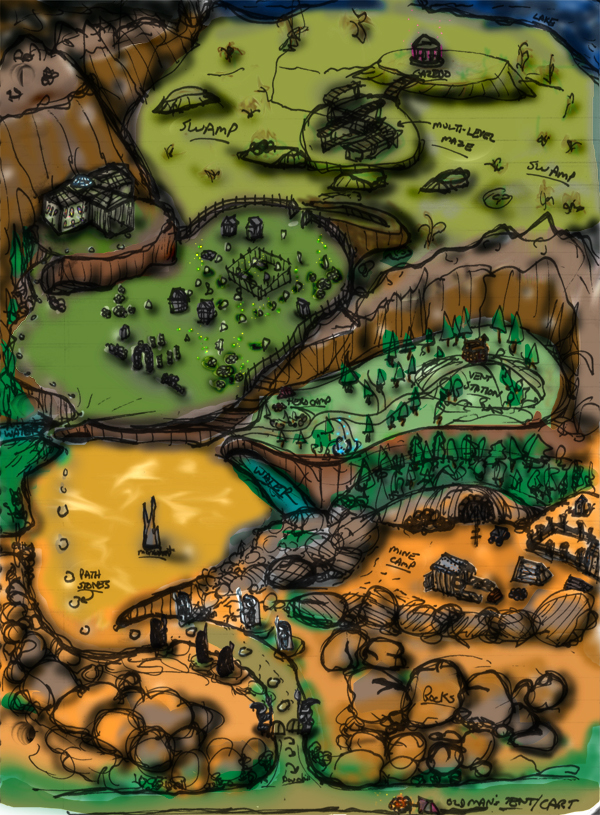
\includegraphics[width=200pt]{images/map_design.jpg}
	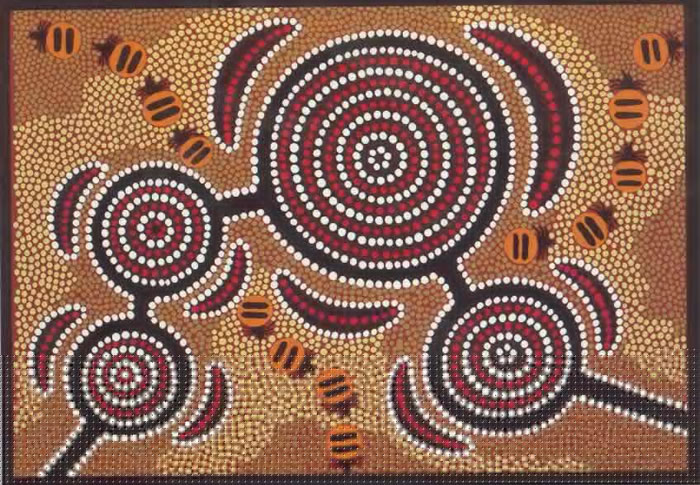
\includegraphics[width=200pt]{images/aboriginal_art.jpg}
	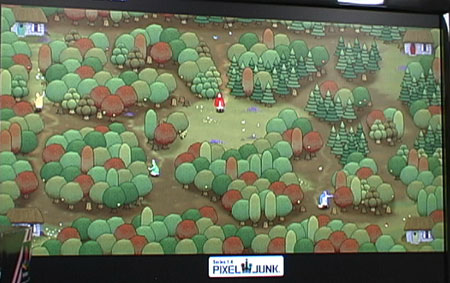
\includegraphics[width=200pt]{images/forest.jpg}
\end{center}
	\caption{impressions}\label{fig:global_map}
\end{figure}


\section{Method: realtime spatial growth models}

\subsection{dynamic structures: polygonal surfaces}
\inhoud{2D polygonale expansie van een ondergrond model als land of water die wordt gestuurd door eigenschappen van het type maar ook door ruimtelijke manipulatie methodes zoals vectorfields. representatie(onder voorbehoud): 
\begin{itemize}
\item Cellular automata
\item Cell systems
\item iets wat niet met cellen werkt  
\end{itemize}
realtime hertriangulatie zal moeten worden toegepast. 
polygonal meshes: 
\begin{itemize}
\item representation for irregular 2D volumes.  
\item suitable for water, land, cave like structures  
\item real-time demand, so need for efficient algorithms
\item houdt rekening met triangulatie
\item houdt rekening met smoothing
\item datastructure
\end{itemize}
citeer: On Vertex-Vertex Systems and Their Use in
Geometric and Biological Modelling
}

\todo{dit kan al snel worden geimplementeerd dus logisch om dit als eerste te beschrijven en methode uit te werken.}

\voegtoe{beschrijf waarom ik dynamic modeling technieken nodig heb}



\voegtoe{review methodes for dynamic modeling}


\voegtoe{focus op cell systems}


\voegtoe{custom systeem dat alle eigenschappen heeft die nodig zijn voor de polygonale expansie}



\cite{compgeom}
\cite{vertexsystems}

\subsection{l-systems and map l-system type spatial growth patterns}

\cite{lcreport}


\subsection{Real-Time spatial growth Models For Outdoor Areas}
\inhoud{Per type spatial growth model bespreken wat de context is binnen outdoor areas en dus met 
welke andere spatial growth modellen het communiceert en welke effecten het spatial growth model heeft 
op de andere en vica versa. Ook bespreken op wat voor manier een vector field (en andere tools 
die invloed hebben op de ruimtelijke indeling)  effect heeft op de uitdijing van dit type model.   
}

\subsubsection{Land} 
\todo{beschrijven hoe land expansie verloopt en hoe het communiceert met andere modellen}

A definition of land: "The part of Earth which is not covered by oceans or other bodies of water".(bron: http://en.wiktionary.org/wiki/land ...jaja ik vind nog wel een betere bron)
In reality land obviously does not grow, so first we must ask ourselves whether growing land in our virtual world can be made useful and intuitive to use. There are no real rules for the bounding shape of a piece of land, the bounds can be configured in any way. However due to this fact almost any random configuration of the shape of land looks realistic. The question is, as with other growth models with a minimum amount of rules, whether generating land by means of a growth model, thereby having less control over the result compared to conventional methods, is something which we want. 

Obviously when you want maximum control over the resulting geometry of a piece of land, using a growth model is not an option. I would like to prove however there are situations in which this method could prove useful. 

\inhoud
{wanneer is het groeien van land handig: 
\begin{itemize}
\item Obviously: In situaties waarin de gebruiker niet veel waarde hecht aan de precieze vorm van de resulterence geometrie.  
\item stimuleert de creativiteit: elaborate. 
\end{itemize}
}

Land provides the underlying surface of many of the growth models discussed in this paper. 

\inhoud
{dus het bestaan van land op de seedpositie van een afhankelijk groeiproces is een eis. Wellicht moet het genereren van een map bestaan uit verschillende fases:
\begin{itemize}
\item fase 1: generatie van land en water. 
\item fase 2: plaatsen en activeren van groei processen die afhankelijk zijn van land.  
\end{itemize}
}

The field of biological modeling provides some interesting modeling techniques for the process of cell division. 
Cell division is interesting with respect to the concept of growing land because it is an expanding process with some nice properties. \voegtoe{benoem properties of revise deze zin.} 


\subsubsection{Water} 

\subsubsection{Roads}

\subsubsection{Afforestation} 

\subsection{Real-time spatial growth models For Indoor Areas}

\subsubsection{Caves}

\subsubsection{Canarian Aboriginal style homes}

\section{Organic map generation tool}

\subsection{Modifiers}

\subsubsection{Spatial modifiers}

\inhoud{
\begin{itemize}
\item vector fields: dit moet je wellicht helemaal aan het begin doen omdat alle spatial growth models
gemanipuleerd worden door deze vector fields.
\item obstruction with solid objects
\item smudge-like tool
\end{itemize}
}

\subsubsection{Timeflow modifiers}
\inhoud{
\begin{itemize}
\item pause model
\item speed up model
\item slow down model
\item reverse time flow
\end{itemize}
}


\subsection{User controlled map generation}

\subsection{automatic map generation} 


\section{Implementation}
\subsection{Tools used}
\inhoud{ 
\begin{itemize}
\item programming language: c++ (for now)
\item visualization library: openGL or Ogre3D (if it features easy vertex manipulation) 
\item physics engine: ODE (onder voorbehoud)  
\item collision detection: D-Collide (onder voorbehoud)
\end{itemize}
}

\subsection{Application Class Structure}

\voegtoe{
klassen structuur(voorlopig):
\begin{itemize}
\item Environment or Canvas: mainloop
\item Seedpoint  
\item GrowthModel 
\item ShapeModel
\item NetworkModel
\item ModelHistory
\item ModelTopology
\item ModelGeometry 
\item EventHandler
\item Communicator
\item Timeline: can place seeds on the timeline which will be handled by eventhandler when time comes.  
\end{itemize}
}






\subsection{User Interface}
\subsection{Communication system between models}

\section{Results}

\section{Conclusion}





%references
%logische volgorde:
%introduction: context-> previous work  
%method
%implementation
%results 
%conclusion 
\newpage 
\bibliographystyle{abbrv}	% (uses file "plain.bst")
\bibliography{thesisrefs}	% expects file "myrefs.bib"

\end{document}

